\documentclass[]{article}
\usepackage{lmodern}
\usepackage{amssymb,amsmath}
\usepackage{ifxetex,ifluatex}
\usepackage{fixltx2e} % provides \textsubscript
\ifnum 0\ifxetex 1\fi\ifluatex 1\fi=0 % if pdftex
  \usepackage[T1]{fontenc}
  \usepackage[utf8]{inputenc}
\else % if luatex or xelatex
  \ifxetex
    \usepackage{mathspec}
  \else
    \usepackage{fontspec}
  \fi
  \defaultfontfeatures{Ligatures=TeX,Scale=MatchLowercase}
\fi
% use upquote if available, for straight quotes in verbatim environments
\IfFileExists{upquote.sty}{\usepackage{upquote}}{}
% use microtype if available
\IfFileExists{microtype.sty}{%
\usepackage{microtype}
\UseMicrotypeSet[protrusion]{basicmath} % disable protrusion for tt fonts
}{}
\usepackage[margin=1in]{geometry}
\usepackage{hyperref}
\hypersetup{unicode=true,
            pdftitle={Introduction to Robust Spatial Extent Inference using the pbj Package},
            pdfauthor={Simon N. Vandekar},
            pdfborder={0 0 0},
            breaklinks=true}
\urlstyle{same}  % don't use monospace font for urls
\usepackage{color}
\usepackage{fancyvrb}
\newcommand{\VerbBar}{|}
\newcommand{\VERB}{\Verb[commandchars=\\\{\}]}
\DefineVerbatimEnvironment{Highlighting}{Verbatim}{commandchars=\\\{\}}
% Add ',fontsize=\small' for more characters per line
\usepackage{framed}
\definecolor{shadecolor}{RGB}{248,248,248}
\newenvironment{Shaded}{\begin{snugshade}}{\end{snugshade}}
\newcommand{\AlertTok}[1]{\textcolor[rgb]{0.94,0.16,0.16}{#1}}
\newcommand{\AnnotationTok}[1]{\textcolor[rgb]{0.56,0.35,0.01}{\textbf{\textit{#1}}}}
\newcommand{\AttributeTok}[1]{\textcolor[rgb]{0.77,0.63,0.00}{#1}}
\newcommand{\BaseNTok}[1]{\textcolor[rgb]{0.00,0.00,0.81}{#1}}
\newcommand{\BuiltInTok}[1]{#1}
\newcommand{\CharTok}[1]{\textcolor[rgb]{0.31,0.60,0.02}{#1}}
\newcommand{\CommentTok}[1]{\textcolor[rgb]{0.56,0.35,0.01}{\textit{#1}}}
\newcommand{\CommentVarTok}[1]{\textcolor[rgb]{0.56,0.35,0.01}{\textbf{\textit{#1}}}}
\newcommand{\ConstantTok}[1]{\textcolor[rgb]{0.00,0.00,0.00}{#1}}
\newcommand{\ControlFlowTok}[1]{\textcolor[rgb]{0.13,0.29,0.53}{\textbf{#1}}}
\newcommand{\DataTypeTok}[1]{\textcolor[rgb]{0.13,0.29,0.53}{#1}}
\newcommand{\DecValTok}[1]{\textcolor[rgb]{0.00,0.00,0.81}{#1}}
\newcommand{\DocumentationTok}[1]{\textcolor[rgb]{0.56,0.35,0.01}{\textbf{\textit{#1}}}}
\newcommand{\ErrorTok}[1]{\textcolor[rgb]{0.64,0.00,0.00}{\textbf{#1}}}
\newcommand{\ExtensionTok}[1]{#1}
\newcommand{\FloatTok}[1]{\textcolor[rgb]{0.00,0.00,0.81}{#1}}
\newcommand{\FunctionTok}[1]{\textcolor[rgb]{0.00,0.00,0.00}{#1}}
\newcommand{\ImportTok}[1]{#1}
\newcommand{\InformationTok}[1]{\textcolor[rgb]{0.56,0.35,0.01}{\textbf{\textit{#1}}}}
\newcommand{\KeywordTok}[1]{\textcolor[rgb]{0.13,0.29,0.53}{\textbf{#1}}}
\newcommand{\NormalTok}[1]{#1}
\newcommand{\OperatorTok}[1]{\textcolor[rgb]{0.81,0.36,0.00}{\textbf{#1}}}
\newcommand{\OtherTok}[1]{\textcolor[rgb]{0.56,0.35,0.01}{#1}}
\newcommand{\PreprocessorTok}[1]{\textcolor[rgb]{0.56,0.35,0.01}{\textit{#1}}}
\newcommand{\RegionMarkerTok}[1]{#1}
\newcommand{\SpecialCharTok}[1]{\textcolor[rgb]{0.00,0.00,0.00}{#1}}
\newcommand{\SpecialStringTok}[1]{\textcolor[rgb]{0.31,0.60,0.02}{#1}}
\newcommand{\StringTok}[1]{\textcolor[rgb]{0.31,0.60,0.02}{#1}}
\newcommand{\VariableTok}[1]{\textcolor[rgb]{0.00,0.00,0.00}{#1}}
\newcommand{\VerbatimStringTok}[1]{\textcolor[rgb]{0.31,0.60,0.02}{#1}}
\newcommand{\WarningTok}[1]{\textcolor[rgb]{0.56,0.35,0.01}{\textbf{\textit{#1}}}}
\usepackage{graphicx,grffile}
\makeatletter
\def\maxwidth{\ifdim\Gin@nat@width>\linewidth\linewidth\else\Gin@nat@width\fi}
\def\maxheight{\ifdim\Gin@nat@height>\textheight\textheight\else\Gin@nat@height\fi}
\makeatother
% Scale images if necessary, so that they will not overflow the page
% margins by default, and it is still possible to overwrite the defaults
% using explicit options in \includegraphics[width, height, ...]{}
\setkeys{Gin}{width=\maxwidth,height=\maxheight,keepaspectratio}
\IfFileExists{parskip.sty}{%
\usepackage{parskip}
}{% else
\setlength{\parindent}{0pt}
\setlength{\parskip}{6pt plus 2pt minus 1pt}
}
\setlength{\emergencystretch}{3em}  % prevent overfull lines
\providecommand{\tightlist}{%
  \setlength{\itemsep}{0pt}\setlength{\parskip}{0pt}}
\setcounter{secnumdepth}{0}
% Redefines (sub)paragraphs to behave more like sections
\ifx\paragraph\undefined\else
\let\oldparagraph\paragraph
\renewcommand{\paragraph}[1]{\oldparagraph{#1}\mbox{}}
\fi
\ifx\subparagraph\undefined\else
\let\oldsubparagraph\subparagraph
\renewcommand{\subparagraph}[1]{\oldsubparagraph{#1}\mbox{}}
\fi

%%% Use protect on footnotes to avoid problems with footnotes in titles
\let\rmarkdownfootnote\footnote%
\def\footnote{\protect\rmarkdownfootnote}

%%% Change title format to be more compact
\usepackage{titling}

% Create subtitle command for use in maketitle
\providecommand{\subtitle}[1]{
  \posttitle{
    \begin{center}\large#1\end{center}
    }
}

\setlength{\droptitle}{-2em}

  \title{Introduction to Robust Spatial Extent Inference using the pbj Package}
    \pretitle{\vspace{\droptitle}\centering\huge}
  \posttitle{\par}
    \author{Simon N. Vandekar}
    \preauthor{\centering\large\emph}
  \postauthor{\par}
      \predate{\centering\large\emph}
  \postdate{\par}
    \date{2019-07-24}

\pdfminorversion=5
\pdfcompresslevel=9
\pdfobjcompresslevel=2

\begin{document}
\maketitle

\hypertarget{acknowledgements}{%
\subsection{Acknowledgements}\label{acknowledgements}}

I am grateful to Shawn Garbett for his help in the preparation and
debugging of the \texttt{pbj} package and the code and theory for this
vignette, as well as other troubling issues I have not yet experienced
that he is likely to help me with.

\hypertarget{the-pbj-hypothesis-testing-procedures}{%
\subsection{The PBJ hypothesis testing
procedures}\label{the-pbj-hypothesis-testing-procedures}}

Spatial extent inference (SEI) is a widely used tool in neuroimaging to
perform group level analysis, where neuroimaging data are modeled as a
function of subject level covariates such as age, sex, diagnosis, and/or
other covariates. The parametric bootstrap joint (PBJ) testing procedure
and the semi-PBJ (sPBJ) are methods that we recently proposed to perform
SEI that relax the assumptions of gaussian random field (GRF) and
permutation based methods. For a detailed description of these
procedures please see (Vandekar, Satterthwaite, Xia, et al. 2018).

The PBJ and sPBJ procedures conceptualize a group level analysis as the
second level in a multilevel model; both allow the user to specify
subject specific weights that can be defined as images (e.g.~varcopes
from fsl) or as a scalar value for each subject. An optimal decision for
the weight for subject \(i\) at voxel \(v\) is the inverse of subject
\(i\)'s variance at location \(v\), call it \(\sigma^{-2}_i(v)\). The
PBJ procedure assumes that the weights the user passes are exactly equal
to \(\sigma^{-2}_i(v)\). However, most of the time, \(\sigma^{-2}_i(v)\)
is unknown. As a solution, the sPBJ procedure uses a robust ``sandwich''
covariance estimator that provides consistent estimates of the standard
errors, even if the estimates of \(\sigma^{-2}_i(v)\) are misspecified.

The sPBJ SEI procedure is appropriate for any type of group level
analysis and we demonstrated that it is robust at cluster forming
thresholds (CFTs) where GRF-based methods fail to control the FWER.

\hypertarget{overview-of-this-vignette}{%
\subsection{Overview of this vignette}\label{overview-of-this-vignette}}

To demonstrate how to use the pbj package, we use data from Maumet et
al. (2016) to perform a meta-analysis of statistical maps from 21 pain
studies (Maumet et al. 2016; Gorgolewski et al. 2015). This vignette
will take you through the process of computing a robust statistical
meta-analytic map from the results of the 21 pain studies, performing
inference on the maps using the PBJ and sPBJ procedures, and saving and
visualizing the results. Note, the \texttt{pbj} analysis package was
designed for group level models where the input data can be subject or
study level data. The tools in this package assume you have fully
processed study (or subject) level imaging data. Preprocessing can be
done using other tools in \texttt{R} (Muschelli et al. 2018).

\begin{figure}
\centering
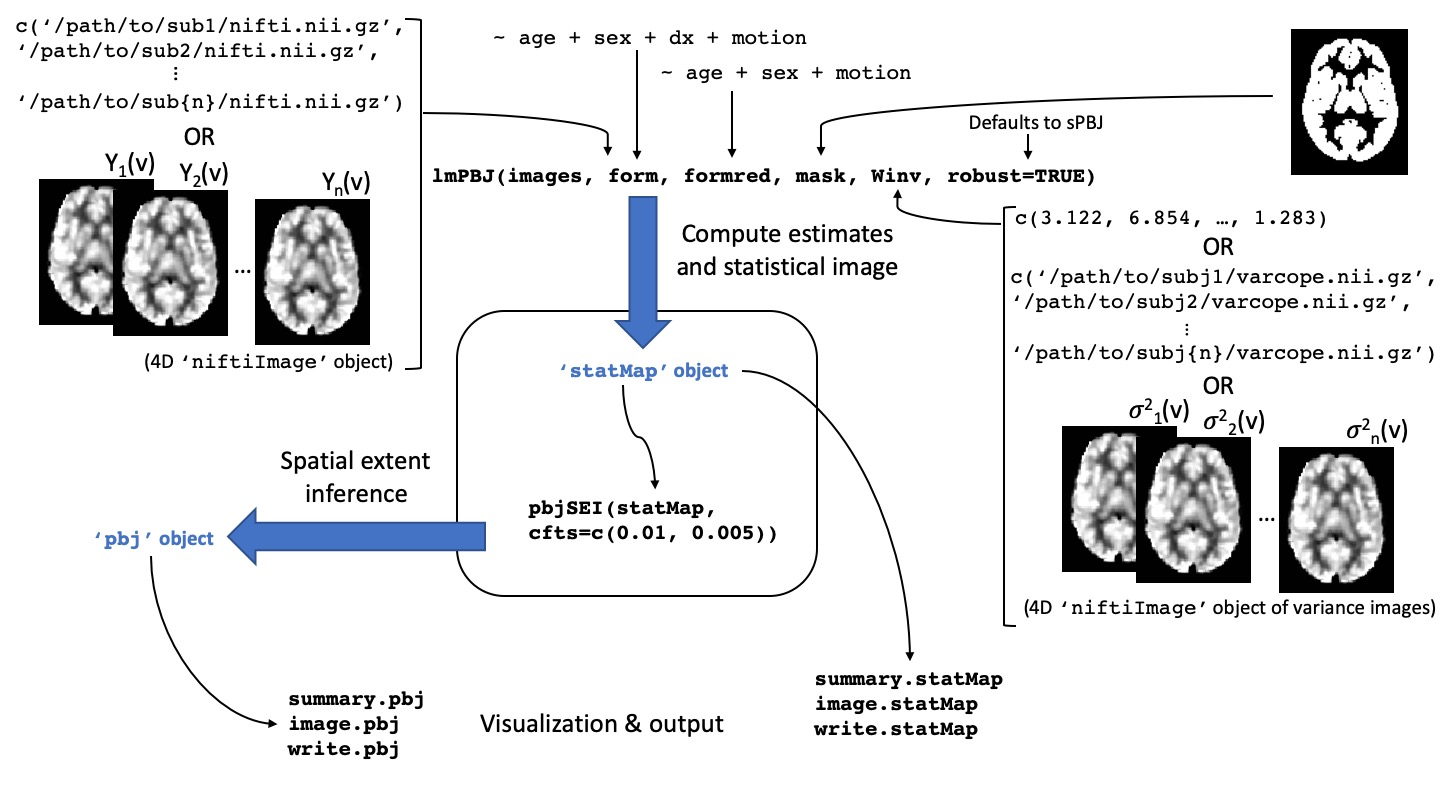
\includegraphics{pbj_schematic.jpg}
\caption{Schematic of pbj analysis functions.}
\end{figure}

\hypertarget{computing-statmaps}{%
\subsection{Computing statMaps}\label{computing-statmaps}}

\hypertarget{loading-in-the-data}{%
\subsubsection{loading in the data}\label{loading-in-the-data}}

The first step is to gather the files we need to perform the analysis.
This is the hardest part; passing the necessary files to the
\texttt{lmPBJ} function produces a \texttt{statMap} object which retains
all of the objects we need to perform SEI and visualization. First, we
install the packages we need. The pain21 package includes curated data
from the ``21 Pain Studies''
\href{https://neurovault.org/collections/1425/}{Neurovault repository}
(Maumet et al. 2016).

\hypertarget{installation}{%
\subsection{INSTALLATION}\label{installation}}

Use these commands:

\begin{verbatim}
install.packages('devtools')
devtools::install_github('simonvandekar/pain21')
devtools::install_github('simonvandekar/pbj')
\end{verbatim}

The \texttt{pain21} function from the \texttt{pain21} package creates a
data frame with file paths for the imaging data that we need to perform
the analysis. The following images are required to perform the analysis:

\begin{itemize}
\tightlist
\item
  The \texttt{mask} image is a binary image indicating which voxels
  should be included in the analysis.
\item
  The character vector of \texttt{images} is the contrast image from
  each study included in the meta-analysis.
\item
  The character vector of \texttt{varimages} contains the voxel level
  estimates of variance from each study.
\end{itemize}

The \texttt{template} is the MNI 152 template and is not necessary to
compute the statistical map or perform SEI, but it is handy to include
here for visualization in later steps.

\begin{Shaded}
\begin{Highlighting}[]
\KeywordTok{library}\NormalTok{(pain21)}
\NormalTok{pain =}\StringTok{ }\KeywordTok{pain21}\NormalTok{()}
\NormalTok{pain}\OperatorTok{$}\NormalTok{mask}
\CommentTok{#> [1] "/Library/Frameworks/R.framework/Versions/3.5/Resources/library/pain21/pain21/mask.nii.gz"}
\KeywordTok{dirname}\NormalTok{(pain}\OperatorTok{$}\NormalTok{data}\OperatorTok{$}\NormalTok{images[}\DecValTok{1}\NormalTok{])}
\CommentTok{#> [1] "/Library/Frameworks/R.framework/Versions/3.5/Resources/library/pain21/pain21"}
\KeywordTok{head}\NormalTok{(}\KeywordTok{basename}\NormalTok{(pain}\OperatorTok{$}\NormalTok{data}\OperatorTok{$}\NormalTok{images))}
\CommentTok{#> [1] "contrast_pain_01.nii.gz" "contrast_pain_02.nii.gz"}
\CommentTok{#> [3] "contrast_pain_03.nii.gz" "contrast_pain_04.nii.gz"}
\CommentTok{#> [5] "contrast_pain_05.nii.gz" "contrast_pain_06.nii.gz"}
\KeywordTok{head}\NormalTok{(}\KeywordTok{basename}\NormalTok{(pain}\OperatorTok{$}\NormalTok{data}\OperatorTok{$}\NormalTok{varimages))}
\CommentTok{#> [1] "var_pain_01.nii.gz" "var_pain_02.nii.gz" "var_pain_03.nii.gz"}
\CommentTok{#> [4] "var_pain_04.nii.gz" "var_pain_05.nii.gz" "var_pain_06.nii.gz"}
\KeywordTok{basename}\NormalTok{(pain}\OperatorTok{$}\NormalTok{template)}
\CommentTok{#> [1] "MNI152_T1_2mm_brain.nii.gz"}
\end{Highlighting}
\end{Shaded}

\hypertarget{computing-the-statistical-map-using-voxel-wise-weights}{%
\subsubsection{Computing the statistical map using voxel-wise
weights}\label{computing-the-statistical-map-using-voxel-wise-weights}}

These data can be passed as arguments to the \texttt{lmPBJ} function.
Since this is a meta-analysis we are performing a one sample t-test, so
the full model includes only the intercept and the reduced model is
\texttt{NULL}. There are many options with how we pass arguments and
analyze the data. As a first pass, we'll use the inverse of the variance
images as weights in the regression. Here, we will specify the outdir
argument, which will save the output as nifti images so that the large
objects stored in the statMap object are not retained in memory. Using
voxel level weights can take a little while because the computation must
be performed separately at each voxel. \texttt{lmPBJ} defaults to using
a robust ``sandwich'' covariance estimate (utilized by the sPBJ
procedure); this can be changed by setting \texttt{robust=FALSE}.
Because we specified the output directory, nifti images of the results
are stored in \texttt{outdir} and \texttt{statmap} includes only
character vectors and formulas that point to the files in
\texttt{outdir}. The output directory and all parent directories are
created automatically by \texttt{lmPBJ}.

\begin{Shaded}
\begin{Highlighting}[]
\KeywordTok{library}\NormalTok{(pbj)}
\CommentTok{# setup model equations}
\NormalTok{form =}\StringTok{ }\ErrorTok{~}\StringTok{ }\DecValTok{1}
\NormalTok{formred =}\StringTok{ }\OtherTok{NULL}
\NormalTok{outdir =}\StringTok{ }\KeywordTok{tempfile}\NormalTok{()}
\KeywordTok{dir.create}\NormalTok{(outdir)}
\end{Highlighting}
\end{Shaded}

\begin{Shaded}
\begin{Highlighting}[]
\NormalTok{comptime =}\StringTok{ }\KeywordTok{system.time}\NormalTok{(}
\NormalTok{  statmap <-}\StringTok{ }\KeywordTok{lmPBJ}\NormalTok{(pain}\OperatorTok{$}\NormalTok{data}\OperatorTok{$}\NormalTok{images, }\DataTypeTok{form =}\NormalTok{ form, }
\NormalTok{                          formred, pain}\OperatorTok{$}\NormalTok{mask,}
                          \DataTypeTok{data =}\NormalTok{ pain}\OperatorTok{$}\NormalTok{data, }
                          \DataTypeTok{Winv =}\NormalTok{ pain}\OperatorTok{$}\NormalTok{data}\OperatorTok{$}\NormalTok{varimages, }\DataTypeTok{outdir=}\NormalTok{outdir)}
\NormalTok{  )}
\CommentTok{#> Weights are voxel-wise.}
\CommentTok{#> Running voxel-wise weighted linear models.}
\CommentTok{#> Getting voxel-wise hat values.}
\CommentTok{#> Getting voxel-wise residuals for covariate and outcome vectors.}
\CommentTok{#> Computing robust stat image.}
\CommentTok{#> Writing output images.}
\CommentTok{#> Writing sqrtSigma 4d image.}

\NormalTok{statmap}
\CommentTok{#> }
\CommentTok{#> Formula: ~1}
\CommentTok{#> }
\CommentTok{#> Contents:}
\CommentTok{#>   Stat:       '/var/folders/h7/d7np_ycn1zs6d9msn4y3r3vr0000gn/T//RtmpV5QeI5/file184059043649/stat.nii.gz' 1.95M}
\CommentTok{#>   Coef:       matrix[1 x 259353]}
\CommentTok{#>   Sqrt Sigma: '/var/folders/h7/d7np_ycn1zs6d9msn4y3r3vr0000gn/T//RtmpV5QeI5/file184059043649/sqrtSigma.nii.gz' 38.22M}
\CommentTok{#>   Mask:       '/Library/Frameworks/R.framework/Versions/3.5/Resources/library/pain21/pain21/mask.nii.gz' 0.02M}
\CommentTok{#>   Robust:     TRUE}
\end{Highlighting}
\end{Shaded}

The summary output gives us an idea of the data we are working with. The
\texttt{lmPBJ} function returns a \texttt{statMap} object, which
contains the following fields:

\begin{itemize}
\tightlist
\item
  The \texttt{stat} object is a character pointing to the statistical
  nifti image
\item
  The \texttt{coef} object is a character pointing to the 4d coefficient
  image
\item
  The \texttt{sqrtSigma} object is a character pointing to a 4d
  covariance nifti image
\item
  The \texttt{mask} object gives the directory to the mask file passed
  as input
\item
  Because we did not specify a template file it does not exist in the
  output
\end{itemize}

\hypertarget{computing-the-statistical-map-with-study-wise-subject-wise-weights}{%
\subsubsection{Computing the statistical map with study-wise
(subject-wise)
weights}\label{computing-the-statistical-map-with-study-wise-subject-wise-weights}}

Often, public data sets only include standardized statistical maps; this
makes meta-analysis using conventional methods (e.g.~mixed effects
models) difficult or impossible because the study level variances aren't
known. However, the sPBJ procedure is still valid in large samples
because it uses robust standard errors, so any weights can be used and
the standard errors are still consistent, as long there is an adequate
number of studies (or subjects) used in the analysis. The best study
level weight is one that is a good estimate of the variance for the
statistical map for that study. However, let's see how inference changes
if we don't have the variance images, but assume instead that the
variance of the estimate from each study is proportional to the square
root of the sample size. The details are not critical to understanding
how to use the package, but feel free to see
\protect\hyperlink{technical_details}{below} for more information.

Let's run this analysis again, instead on scaled versions of the
statistical maps. Instead of voxel-wise weights we'll use weights are
that proportional to the sample size for each study. Because we are now
going to pass statistical maps to \texttt{lmPBJ}, we will compute these
maps in \texttt{R} and pass \texttt{niftiImage} objects as arguments to
\texttt{lmPBJ}, instead of character vectors. Note that we are passing
the weights using the \texttt{W=} argument this time because the weights
are assumed to be approximately inversely proportional to the variance.
We include the \texttt{template} argument here for downstream
aesthetics.

\begin{Shaded}
\begin{Highlighting}[]
\KeywordTok{library}\NormalTok{(pbj)}
\CommentTok{# formulas can be passed as strings}
\NormalTok{form =}\StringTok{ '~ 1'}
\NormalTok{formred =}\StringTok{ }\OtherTok{NULL}

\KeywordTok{library}\NormalTok{(RNifti) }\CommentTok{# NIfTI IO}
\KeywordTok{library}\NormalTok{(abind)  }\CommentTok{# to concatenate 4d arrays}
\CommentTok{# read in contrast images}
\NormalTok{images =}\StringTok{ }\KeywordTok{readNifti}\NormalTok{(pain}\OperatorTok{$}\NormalTok{data}\OperatorTok{$}\NormalTok{images)}
\CommentTok{# read in variance images}
\NormalTok{varimages =}\StringTok{ }\KeywordTok{readNifti}\NormalTok{(pain}\OperatorTok{$}\NormalTok{data}\OperatorTok{$}\NormalTok{varimages)}

\CommentTok{# images gets the statistical images scaled by sample size}
\NormalTok{images =}\StringTok{ }\KeywordTok{lapply}\NormalTok{(}\DecValTok{1}\OperatorTok{:}\KeywordTok{length}\NormalTok{(images), }\ControlFlowTok{function}\NormalTok{(ind)\{}
  \CommentTok{# get stat image}
\NormalTok{  out =}\StringTok{ }\NormalTok{images[[ind]];}
  \CommentTok{# scale out variance and sample size}
\NormalTok{  out[ varimages[[ind]]}\OperatorTok{!=}\DecValTok{0}\NormalTok{] =}\StringTok{  }\NormalTok{out[ varimages[[ind]]}\OperatorTok{!=}\DecValTok{0}\NormalTok{ ] }\OperatorTok{/}\StringTok{ }\KeywordTok{sqrt}\NormalTok{(varimages[[ind]][ varimages[[ind]]}\OperatorTok{!=}\DecValTok{0}\NormalTok{] }\OperatorTok{*}\StringTok{ }\NormalTok{pain}\OperatorTok{$}\NormalTok{data}\OperatorTok{$}\NormalTok{n[ind]);}
\NormalTok{  out\})}

\CommentTok{# don't need these anymore}
\KeywordTok{rm}\NormalTok{(varimages)}

\CommentTok{# create 4d nifti image of study level statistical maps}
\NormalTok{images =}\StringTok{ }\KeywordTok{updateNifti}\NormalTok{(}\KeywordTok{do.call}\NormalTok{(abind, }\KeywordTok{c}\NormalTok{(images, }\DataTypeTok{along=}\DecValTok{4}\NormalTok{)), }\KeywordTok{readNifti}\NormalTok{(pain}\OperatorTok{$}\NormalTok{template))}

\CommentTok{# third level analysis of statistical maps}
\NormalTok{comptimen =}\StringTok{ }\KeywordTok{system.time}\NormalTok{(statmapn <-}\StringTok{ }\KeywordTok{lmPBJ}\NormalTok{(images, form, formred, pain}\OperatorTok{$}\NormalTok{mask,}
                                                 \DataTypeTok{template=}\NormalTok{pain}\OperatorTok{$}\NormalTok{template, }\DataTypeTok{data =}\NormalTok{ pain}\OperatorTok{$}\NormalTok{data, }\DataTypeTok{W =}\NormalTok{ pain}\OperatorTok{$}\NormalTok{data}\OperatorTok{$}\NormalTok{n))}
\CommentTok{#> Performing voxel regression.}
\CommentTok{#> Computing hat values.}
\CommentTok{#> Getting residuals}
\CommentTok{#> Computing robust stat image.}

\NormalTok{statmapn}
\CommentTok{#> }
\CommentTok{#> Formula: ~ 1}
\CommentTok{#> }
\CommentTok{#> Contents:}
\CommentTok{#>   Stat:       matrix[1 x 259353]}
\CommentTok{#>   Coef:       matrix[1 x 259353]}
\CommentTok{#>   Sqrt Sigma: matrix[259353 x 21]}
\CommentTok{#>   Mask:       nifti[91 x 109 x 91] Pixel dimensions: 2mm x 2mm x 2s}
\CommentTok{#>   Template:   '/Library/Frameworks/R.framework/Versions/3.5/Resources/library/pain21/pain21/MNI152_T1_2mm_brain.nii.gz' 0.39M}
\CommentTok{#>   Robust:     TRUE}
\end{Highlighting}
\end{Shaded}

The statistical map with study level weights has a much faster compute
time than the voxel-wise weights because the voxel-wise weights require
inverting a matrix at each location in the mask, whereas the study level
weights only need to invert one matrix. In our paper, for group level
analyses of subject level data, motion was a very effective estimate of
subject level variance (Vandekar, Satterthwaite, Xia, et al. 2018). We
will see here that our sample size approximation leads to reductions in
power.

The \texttt{statMap} object has a slightly different output here because
we did not specify an output directory.

\begin{itemize}
\tightlist
\item
  The \texttt{stat} object is \(V\)-vector, where \(V\) is the number of
  nonzero voxels in the mask, indicating the statistical values within
  the mask
\item
  The \texttt{coef} object is a \(m_1 \times V\) matrix, where \(m_1\)
  is the number of extra parameters in the full model, giving the
  parameter estimates
\item
  The \texttt{sqrtSigma} object is a \(V \times n\) matrix that is a
  square root of the covariance matrix of the test-statistics
\item
  The \texttt{mask} is a niftiImage object of the mask file
\item
  The \texttt{template} object is a character of the template file
\end{itemize}

\texttt{statMap} includes other things that are important to keep track
of, such as the formulas used in the call to \texttt{lmPBJ}, whether the
robust covariance was used, the degrees of freedom, and residual degrees
of freedom. By default, for 1-dimensional parameter images
(i.e.~t-tests) a Z-statistic image is return for the \texttt{stat}
object. This is encoded within the \texttt{pbj} package by setting
\texttt{statmap\$df=0}.

Although, the \texttt{pbj} procedures do not make assumptions about the
distribution of the errors we still transform the T-statistics to
Z-statistics and the F-statistics to Chi-square statistics (for details
see Vandekar, Satterthwaite, Rosen, et al. 2018). We have found that
this improves small sample performance in simulations.

\hypertarget{visualizing-and-saving-statmap-objects}{%
\subsubsection{\texorpdfstring{Visualizing and saving \texttt{statMap}
objects}{Visualizing and saving statMap objects}}\label{visualizing-and-saving-statmap-objects}}

At this point we may want to view the statistical images to see what the
results look like at a few different CFTs. We can do this using
\texttt{statMap} method for the \texttt{image} function. The default
threshold for visualization is 2.32, which is a one-sided p-value of
approximately 0.01.

\begin{Shaded}
\begin{Highlighting}[]
\CommentTok{#image(statmap)}
\KeywordTok{image}\NormalTok{(statmapn)}
\end{Highlighting}
\end{Shaded}

\begin{figure}
\centering
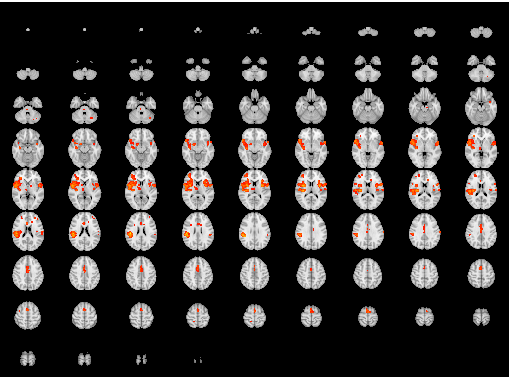
\includegraphics{introduction_to_pbj_files/figure-latex/unnamed-chunk-6-1.pdf}
\caption{A comparison of using voxel-wise level standard error estimates
for parameter estimates versus using study-level standard error
estimates based on sample size.}
\end{figure}

We can see from the maps that using voxel-level weights appears to be
more powerful: there are more extreme values. Because we did not specify
a template image for the first analysis, image defaults to plotting on
the mask image. If no mask image is passed then \texttt{pbjSEI} will
error.

It is also possible to display the lightbox for other orientations:

\begin{Shaded}
\begin{Highlighting}[]
\CommentTok{#image(statmap, plane='coronal')}
\KeywordTok{image}\NormalTok{(statmapn, }\DataTypeTok{plane=}\StringTok{'sagittal'}\NormalTok{)}
\end{Highlighting}
\end{Shaded}

\begin{figure}
\centering
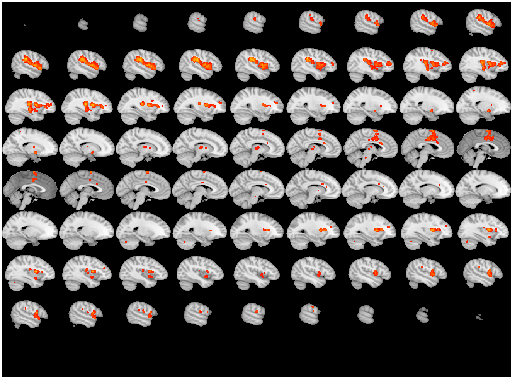
\includegraphics{introduction_to_pbj_files/figure-latex/unnamed-chunk-8-1.pdf}
\caption{Other image views.}
\end{figure}

the function \texttt{write.statMap} can be used to write the output to a
directory for later use (e.g.~separate visualization or to upload to a
public access database).

\begin{Shaded}
\begin{Highlighting}[]
\NormalTok{resdir =}\StringTok{ }\KeywordTok{tempfile}\NormalTok{()}
\KeywordTok{dir.create}\NormalTok{(resdir)}
\KeywordTok{write.statMap}\NormalTok{(statmapn, }\DataTypeTok{outdir=}\NormalTok{resdir)}
\CommentTok{#> Writing output images.}
\CommentTok{#> Writing sqrtSigma 4d image.}
\CommentTok{#> $stat}
\CommentTok{#> [1] "/var/folders/h7/d7np_ycn1zs6d9msn4y3r3vr0000gn/T//RtmpV5QeI5/file1840554ef020/stat.nii.gz"}
\CommentTok{#> }
\CommentTok{#> $coef}
\CommentTok{#> [1] "/var/folders/h7/d7np_ycn1zs6d9msn4y3r3vr0000gn/T//RtmpV5QeI5/file1840554ef020/coef.nii.gz"}
\CommentTok{#> }
\CommentTok{#> $sqrtSigma}
\CommentTok{#> [1] "/var/folders/h7/d7np_ycn1zs6d9msn4y3r3vr0000gn/T//RtmpV5QeI5/file1840554ef020/sqrtSigma.nii.gz"}
\end{Highlighting}
\end{Shaded}

\hypertarget{performing-sei-on-the-statmap-objects}{%
\subsection{\texorpdfstring{Performing SEI on the \texttt{statMap}
objects}{Performing SEI on the statMap objects}}\label{performing-sei-on-the-statmap-objects}}

The next step is to perform spatial extent inference to see how likely
our results are to have occurred under the global null hypothesis that
the image is not associated with the covariate. In this case, the global
null corresponds to the hypothesis that the mean of the study-level
images is equal to zero.

\hypertarget{performing-sei-using-pbjsei}{%
\subsubsection{\texorpdfstring{Performing SEI using
\texttt{pbjSEI}}{Performing SEI using pbjSEI}}\label{performing-sei-using-pbjsei}}

The \texttt{statMap} object includes the statistical map
(\texttt{statmap\$stat}) and a matrix that is proportional to an
estimate of a square root of the covariance matrix of the statistical
map (\texttt{statmap\$sqrtSigma}). The \texttt{sqrtSigma} object can be
use to estimate the distribution of the largest cluster size under the
null using a parametric bootstrap procedure (Vandekar, Satterthwaite,
Xia, et al. 2018). This distribution is then used to compute p-values
for each cluster.

This step is easy to evaluate because the \texttt{statMap} object
contains all of the objects necessary to perform SEI on the statistical
map. The only thing we need to do is specify the CFTs. We have the voxel
level map, which we might choose to use a more stringent threshold on to
get finer anatomical details, so we might lean towards a CFT of 0.005.
For the study level map we've lost some power with our approximation, so
we get anatomically distinct clusters at a lower threshold, so we might
lean towards a CFT of 0.01. The default is to use multiple CFTs,
\texttt{cfts=c(0.01,\ 0.005)}, which will run the sPBJ procedure at both
thresholds.

Under the hood, the clustering procedure operates using a large sample
Chi-square approximation, even for t-tests. It does this by squaring the
To be consistent with other neuroimaging software, the CFT for t-tests
assumes a 1-tailed test. We do this by multiplying the CFT by 2 in the
case that a t-test was performed, which is encoded in the
\texttt{statMap} by \texttt{statMap\$df=0}.

Because the PBJ and sPBJ procedures use a bootstrap, the \texttt{nboot}
argument can be used to control the number of bootstrap samples used.
For this example we use 200 samples, but for a publication a few
thousand is more appropriate to reduce the error in the computational
approximation. \texttt{pbjSEI} keeps track of progress while it's
running (not shown here). We again use \texttt{system.time} here to
track computing times.

\begin{Shaded}
\begin{Highlighting}[]
\NormalTok{pbjcomptime  =}\StringTok{ }\KeywordTok{system.time}\NormalTok{(sPBJ  <-}\StringTok{ }\KeywordTok{pbjSEI}\NormalTok{(statmap,  }\DataTypeTok{nboot=}\DecValTok{200}\NormalTok{))}
\NormalTok{pbjcomptimen =}\StringTok{ }\KeywordTok{system.time}\NormalTok{(sPBJn <-}\StringTok{ }\KeywordTok{pbjSEI}\NormalTok{(statmapn, }\DataTypeTok{nboot=}\DecValTok{200}\NormalTok{))}
\end{Highlighting}
\end{Shaded}

The bootstrap time doesn't differ between voxel-wise or study/subject
level weights.

\begin{Shaded}
\begin{Highlighting}[]
\KeywordTok{print}\NormalTok{(}\KeywordTok{c}\NormalTok{(}\StringTok{'voxel weights'}\NormalTok{=pbjcomptime[}\DecValTok{3}\NormalTok{], }\StringTok{'study weights'}\NormalTok{=pbjcomptimen[}\DecValTok{3}\NormalTok{]))}
\CommentTok{#> voxel weights.elapsed study weights.elapsed }
\CommentTok{#>                51.448                45.294}
\end{Highlighting}
\end{Shaded}

The \texttt{pbjSEI} function returns a \texttt{pbj} object which
contains information about which clusters are large enough to be
unlikely to have occurred by chance under the global null. This object
is a list containing the following things:

\begin{itemize}
\tightlist
\item
  \texttt{stat} This is the statistical map from the \texttt{statMap}
  object without changes
\item
  \texttt{template} This is the template you passed to the
  \texttt{statMap} object
\item
  \texttt{mask} This is the mask image from the \texttt{statMap} object
  without changes
\item
  \texttt{cft*} This is a list containing the following:

  \begin{itemize}
  \tightlist
  \item
    \texttt{pvalues} This is a vector of the SEI p-values, ordered
    relative to space, not value
  \item
    \texttt{clustmap} This is a \texttt{niftiImage} object of cluster
    indices where each index in \texttt{clustmap} corresponds to that
    particular index of the vector of SEI p-values
  \item
    \texttt{pmap} This is a \texttt{niftiImage} object of
    \texttt{-log10(p)} where \texttt{p} is the SEI p-value
  \end{itemize}
\end{itemize}

\hypertarget{visualizing-and-saving-pbj-objects}{%
\subsubsection{Visualizing and saving pbj
objects}\label{visualizing-and-saving-pbj-objects}}

\texttt{pbj} objects can be visualized in the same way as the
\texttt{statMap} object. The image function takes a desired rejection
threshold \texttt{alpha} and only plots clusters with cluster-wise
p-values below that threshold.

If multiple CFTs were used it produces the images for each of those
thresholds.

\begin{Shaded}
\begin{Highlighting}[]
\KeywordTok{image}\NormalTok{(sPBJn, }\DataTypeTok{alpha =} \FloatTok{0.2}\NormalTok{)}
\end{Highlighting}
\end{Shaded}

The \texttt{write.pbj} function can be used to export the the images
contained in the \texttt{pbj} object and save summary results in a .csv
file. The cluster and p-value maps are written for every CFT in a
standardized format \texttt{pbj\_sei\_clust\_cft*.nii.gz} and
\texttt{pbj\_sei\_log10p\_cft*.nii.gz}, respectively.

\begin{Shaded}
\begin{Highlighting}[]
\KeywordTok{write.pbj}\NormalTok{(sPBJn, resdir)}
\end{Highlighting}
\end{Shaded}

\begin{Shaded}
\begin{Highlighting}[]
\NormalTok{tab =}\StringTok{ }\KeywordTok{read.table}\NormalTok{(}\KeywordTok{file.path}\NormalTok{(resdir, }\StringTok{'sei_table_cft0.01.csv'}\NormalTok{), }\DataTypeTok{check.names =} \OtherTok{FALSE}\NormalTok{, }\DataTypeTok{sep =} \StringTok{','}\NormalTok{, }\DataTypeTok{header=}\OtherTok{TRUE}\NormalTok{, }\DataTypeTok{as.is =} \OtherTok{TRUE}\NormalTok{)}
\KeywordTok{head}\NormalTok{(tab)}
\CommentTok{#>   Index Adjusted p-value Signed log10(p-value) Volume (mm)   Centroid}
\CommentTok{#> 1     6        0.1641791             0.7846821       23112 44, -4, 11}
\CommentTok{#> 2    22        0.5024876             0.2988747        2304  -55, 4, 6}
\CommentTok{#> 3    24        0.5174129             0.2861627        2144 -35, 9, 12}
\CommentTok{#> 4     4        0.5671642             0.2462912        1712  2, -1, 42}
\CommentTok{#> 5     1        0.6517413             0.1859248        1104   1, 3, 64}
\CommentTok{#> 6    31        0.7810945             0.1072964         448 -42, 4, -8}
\end{Highlighting}
\end{Shaded}

\hypertarget{simulation-tools}{%
\subsection{Simulation tools}\label{simulation-tools}}

Tools to run simulations as in (Vandekar, Satterthwaite, Xia, et al.
2018) are in progress.

\hypertarget{appendix}{%
\subsection{Appendix}\label{appendix}}

\hypertarget{glossary-of-acronyms}{%
\subsubsection{Glossary of acronyms}\label{glossary-of-acronyms}}

\begin{itemize}
\tightlist
\item
  CFT - cluster forming threshold. The threshold chosen to binarize the
  statistical map for spatial extent hypothesis testing.
\item
  PBJ - parametric bootstrap joint (testing procedure).
\item
  sPBJ - semiparametric bootstrap joint (testing procedure). Robust to
  variance misspecification.
\item
  SEI - spatial extent inference. Using thresholded contiguous cluster
  extents to perform inference on a statistical map.
\end{itemize}

\hypertarget{technical-details-for-study-level-weights}{%
\subsubsection{Technical details for study level
weights}\label{technical-details-for-study-level-weights}}

Because fMRI data are in arbitrary units, one parameter of interest may
be a standardized parameter estimate. For each study \(i=1, \ldots, 21\)
\[ \mathbb{E} Z_i = \mathbb{E} \left\{\left(\frac{\hat{\beta}_i}{ \hat{\sigma}_{yi}}\right) \times (X_{ri}^TX_{ri})^{1/2} \right\}
\approx \left(\frac{\beta}{\sigma_{yi}}\right) \times \mathbb{E}\left\{(X_{ri}^TX_{ri})^{1/2} \right\} \approx \left(\frac{\beta}{\sigma_{yi}} \right) \times \sqrt{n_i},\]
where \(\sigma^2_{yi}\) is the variance for the subjects \(y\) from
study \(i\), \(\beta\) is the unknown parameter, and \(X_{ri}\) is the
vector for the covariate of interest (pain scale for study \(i\)). The
first approximation is because the function in the expectation is
nonlinear; also, because scaling \(X_{ri}\) differently for each study
proportionally changes the scale of \(\hat \beta_i\), so we assume that,
across data sets, the scaling of \(X_{ri}\) is constant so that the
expectation \(\mathbb{E}\{\hat{\beta}_i\}\) does not depend on \(i\),
and the scale of
\(\mathbb{E}\left\{(X_{ri}^TX_{ri})^{1/2} \right\} = O(\sqrt{n_i})\)
only depends on the sample size. Because we are assuming \(\sigma_{yi}\)
are not provided we further assume \(\sigma_{yi} = \sigma_y\).

We can obtain estimates of \(\frac{\beta}{\sigma_y}\) from \[
\mathbb{E}n_i^{-1/2}Z_i \approx \left(\frac{\beta}{\sigma_{yi}} \right),
\] and then weight with \(n_i\) since \[
\text{Var}(n_i^{-1/2} Z_i) = n_i^{-1}.
\] \protect\hyperlink{technical_details_return}{Back} to ``Computing the
statistical map with study-wise (subject-wise) weights''

\hypertarget{references}{%
\subsection*{References}\label{references}}
\addcontentsline{toc}{subsection}{References}

\hypertarget{refs}{}
\leavevmode\hypertarget{ref-gorgolewski_neurovault.org:_2015}{}%
Gorgolewski, Krzysztof J., Gael Varoquaux, Gabriel Rivera, Yannick
Schwarz, Satrajit S. Ghosh, Camille Maumet, Vanessa V. Sochat, et al.
2015. ``NeuroVault.Org: A Web-Based Repository for Collecting and
Sharing Unthresholded Statistical Maps of the Human Brain.''
\emph{Frontiers in Neuroinformatics} 9.
\url{https://doi.org/10.3389/fninf.2015.00008}.

\leavevmode\hypertarget{ref-maumet_sharing_2016}{}%
Maumet, Camille, Tibor Auer, Alexander Bowring, Gang Chen, Samir Das,
Guillaume Flandin, Satrajit Ghosh, et al. 2016. ``Sharing Brain Mapping
Statistical Results with the Neuroimaging Data Model.'' \emph{Scientific
Data} 3 (December). \url{https://doi.org/10.1038/sdata.2016.102}.

\leavevmode\hypertarget{ref-muschelli_neuroconductor:_2018}{}%
Muschelli, John, Adrian Gherman, Jean-Philippe Fortin, Brian Avants,
Brandon Whitcher, Jonathan D. Clayden, Brian S. Caffo, and Ciprian M.
Crainiceanu. 2018. ``Neuroconductor: An R Platform for Medical Imaging
Analysis.'' \emph{Biostatistics}.
\url{https://doi.org/10.1093/biostatistics/kxx068}.

\leavevmode\hypertarget{ref-vandekar_faster_2018}{}%
Vandekar, Simon N., Theodore D. Satterthwaite, Adon Rosen, Rastko Ciric,
David R. Roalf, Kosha Ruparel, Ruben C. Gur, Raquel E. Gur, and Russell
T. Shinohara. 2018. ``Faster Family-Wise Error Control for Neuroimaging
with a Parametric Bootstrap.'' \emph{Biostatistics} 19 (4): 497--513.
\url{https://doi.org/10.1093/biostatistics/kxx051}.

\leavevmode\hypertarget{ref-vandekar_robust_2018}{}%
Vandekar, Simon N., Theodore D. Satterthwaite, Cedric H. Xia, Kosha
Ruparel, Ruben C. Gur, Raquel E. Gur, and Russell T. Shinohara. 2018.
``Robust Spatial Extent Inference with a Semiparametric Bootstrap Joint
Testing Procedure.'' \emph{arXiv:1808.07449 {[}Stat{]}}, August.
\url{http://arxiv.org/abs/1808.07449}.


\end{document}
